\documentclass{article}
\usepackage{amsmath}
\usepackage{amssymb}
\usepackage{graphicx}
\usepackage{hyperref}
\usepackage[version=4]{mhchem}

\title{Example 15}
\date{}

\begin{document}
\maketitle

The measures of the sides of a right triangle are 60, 80, and 100. Find the measure of a line segment, drawn from the vertex of the right angle to the hypotenuse, that divides the triangle into two triangles of equal perimeters.

Solution:
Let \(A B=60, A C=80\), and \(B C=100\). If \(\triangle A B D\) is to have the same perimeter as \(\triangle A C D\), then \(A B+B D\) must equal \(A C+D C\), since both triangles share \(A D\); that is, \(60+B D=80+100-\) \(B D\). Therefore, \(B D=60\) and \(D C=40\).\\
Draw \(D E\) perpendicular to \(A C\).\\
Right \(\triangle E D C \sim\) right \(\triangle A B C\); therefore, \(\frac{E D}{A B}=\frac{D C}{B C}\).\\
\centering
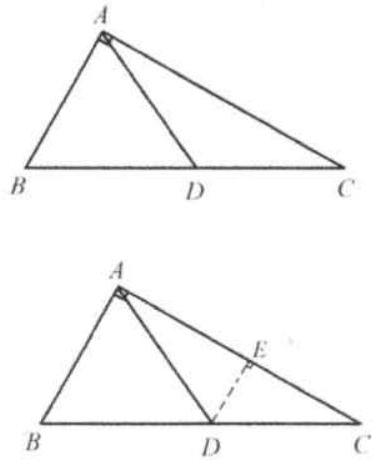
\includegraphics[width=\textwidth]{images/083(2).jpg}


By substituting the appropriate values, we have \(\frac{E D}{60}=\frac{40}{100}\), and \(E D=24\).

By the Pythagorean Theorem, for \(\triangle E D C\), we find \(E C=32\); then, by subtraction, \(A E=48\). Again, using the Pythagorean Theorem, in \(\triangle A E D, A D=24 \sqrt{5}\).


\end{document}
